\documentclass[crop,tikz]{standalone}% 'crop' is the default for v1.0, before it was 'preview'
\usepackage{graphicx}% Include figure files
\usepackage{hyperref}% add hypertext capabilities
\usepackage{subfig}
\usepackage{mathptmx}
\usepackage{microtype}
\usepackage{pgfplots, pgfplotstable}
\usepgfplotslibrary{fillbetween}
\pgfplotsset{compat=1.15} 
\begin{document}
  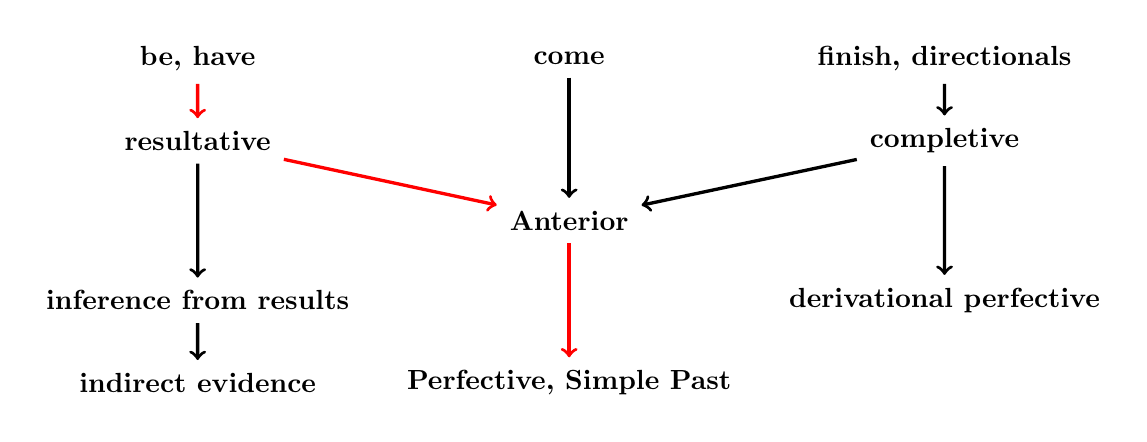
\begin{tikzpicture}[scale=.75]
    \tikzstyle{ann} = [draw=none,fill=none,right]
    \matrix (m) [nodes={draw, thick, fill=blue!10},
    row sep=0.5cm,column sep=0.5cm] {
      % 9 wide matrix; here comes first line:
      \node(A1) [draw=none,fill=none]{\textbf{be, have}};    & \node(A2) [draw=none,fill=none]{\textbf{come}};       & \node(A3) [draw=none,fill=none]{\textbf{finish, directionals}};\\
      \node(B1) [draw=none,fill=none]{\textbf{resultative}}; &                   & \node(B3) [draw=none,fill=none]{\textbf{completive}};\\
      \node [draw=none,fill=none]{};                     & \node(C2) [draw=none,fill=none]{\textbf{Anterior}};   & \\
      \node(D1) [draw=none,fill=none]{\textbf{inference from results}}; &           & \node(D3) [draw=none,fill=none]{\textbf{derivational perfective}};\\
      \node(E1) [draw=none,fill=none]{\textbf{indirect evidence}};  & \node(E2) [draw=none,fill=none]{\textbf{Perfective, Simple Past}}; \\ 
   };
   \path[->,  shorten <=1pt, shorten >=1pt, very thick]
   % % arrows for first line:
   (A1) edge[color=red] (B1)
   (B1) edge (D1)
   (D1) edge (E1)
   (A2) edge (C2)
   (C2) edge[red] (E2)
   (A3) edge (B3)
   (B3) edge (D3)
   (B1) edge[red] (C2)
   (B3) edge (C2);
 \end{tikzpicture}
\end{document}
%%% Local Variables:
%%% mode: latex
%%% TeX-master: t
%%% End:
